\subsection{Toolkit introduction}
4 components, what should it do (online/offline), image2image, gal2gal, cat2cat, albert drawing

\begin{figure}[htb]
  \centering
  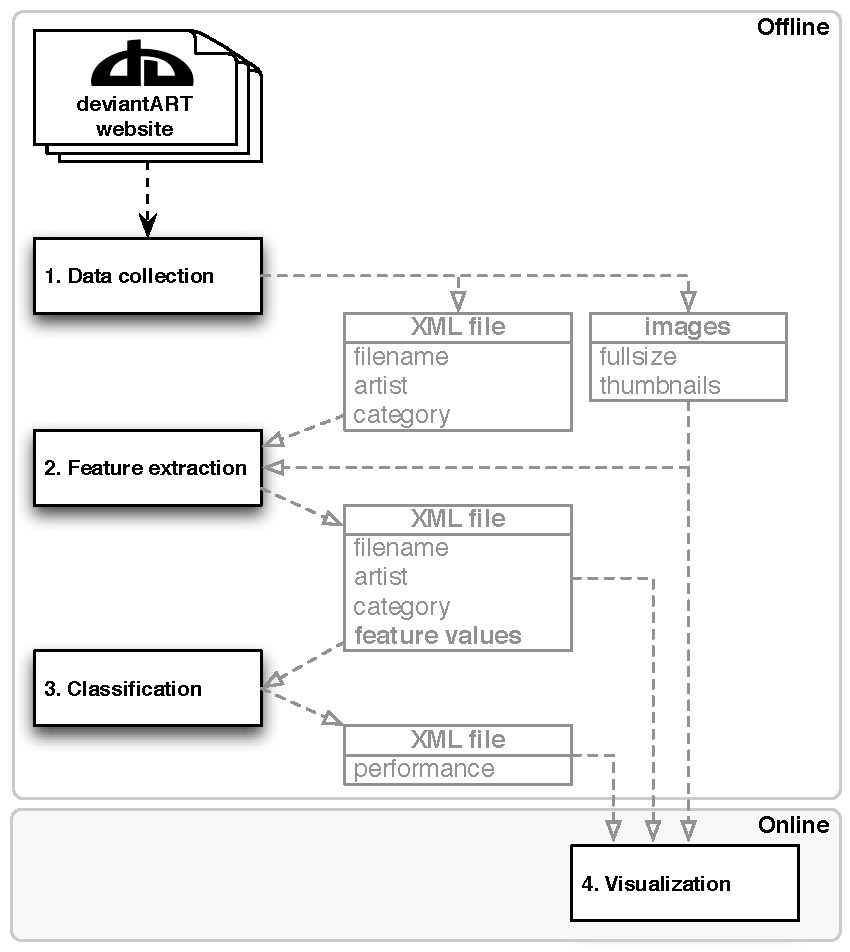
\includegraphics[width=1\linewidth]{img/components.pdf}
  \caption{Interaction between the four components of the toolkit.}
  \label{fig:components}
\end{figure}

\subsection{Data collection}
\subsection{Feature extraction}
\subsection{Classification}
\subsection{Visualization}

% toolboxes used
\subsection{Data collection}
[Sander, Bart B.]
% xml format
% network

DeviantArt provides users, also called deviants, galleries of their images. 
When someone visits such a gallery a featured page will be shown. Furthermore
the user is provided with options to browse the gallery or visit a sub gallery
defined by the user. There are various types of members: normal members, premium 
members, banned members, staff members, etc. Premium members have extra benefits
like no ads, gallery customization, beta-test new site features and more.

DeviantArt does not provide a web api to download images. This makes it more 
difficult to download images. On top of that changes to the website can possible break
down the downloading application.

DeviantArt does provide rss, which allows us to download xml files containing 
information about the users galleries. RSS XML files are more easy to parse
than the html gallery pages.

For each image the full sized image and two different sized thumbnails are 
available. DeviantArt supports png, jpeg, bmp and gif image formats.

For the data collection of the galleries we followed the backend links to
the RSS XML files. Our \textit{scraper} is implemented in python and uses
built-in libraries to parse the XML files. For each image we stored general 
information like the category, deviantART link and filename and we downloaded
the full image and the thumbnails.

For the network information collection we parsed the HTML watchers pages
of the users, since no RSS XML files are provided by deviantART for this
information.

\subsection{Feature extraction}
When working with images, it is usually not possible to work with the raw image data (the pixel values). The reason for this is the high dimensionality of images, which can easily exist in a space of more than a million dimensions. By extracting features from images, they can be represented in a lower dimensional feature-space.  This feature extraction process has several advantages:
\begin{itemize}
\item The data becomes computationally easier to work with due to the smaller number of dimensions
\item By using the right features, the data becomes more suitable for generalization across images
\item Reducing the dimensionality makes it easier to visualize sets of images
\item Features can have an intuitive basis, which makes it easier for non-computer-scientists to analyze (sets of) images
\end{itemize}
\textit{Here something general about different kinds of image features}

% Computer vision is an important and maturing engineering science. It underpins an increasing variety of applications that require the acquisition, analysis, and interpretation of visual information.
In the extraction of image features, a distinction was made between low-level statistical features and higher level cognitive-based features....

\subsubsection{Statistical features}
As statistical features, many relatively simple low-level features were extracted from the images.
The first type of statistical features that were used are color-based features, which should capture the color-usage in the artwork. Many artists produce collections of art pieces with similar colors, and should therefore be (partially) distinguishable with color-based features. For each of the three RGB channels, an average and median is calculated over all the channel values. The image is also converted into the HSV color space, from which the average and median Hue, Saturation and Value are extracted.  

The second group of features is the edge to pixel and corner to pixel ratio. The edge to pixel ratio is calculated by performing Canny edge detection on the image to construct an image of edges. The number of edge pixels in this image, divided by the total number of pixels is then used as a feature. The same is done using a corner detector. These two features should be helpful in distinguishing many photography artwork from other genres such as cartoons and manga. The latter two tend to have large patches of plain color patches, which will decrease the amount of edges and corners. They are also somewhat indicative to the type of scenes in photography. A blue sky will not contain produce many edges or corners, whereas a busy street will.     


%\begin{itemize}
%\item Edge ratio: description
%\item Corner ratio: description
%\item etc...
%\end{itemize}
\subsubsection{Weibull, this subsubsubsection can be made normal text, but we can do that later}
The contrast of natural image statistics has been shown to conform to Weibull-shaped probability distributions \cite{Weibull_physical}. Furthermore, when images do not adhere to this distribution, the images in question are mashups of multiple sub-images which themselves do conform to the Weibull distribution. In addition to this property of natural images, it has been proposed that the parameters for the Weibull distribution form a basis for the description of texture in images \cite{Weibull_6}. There is indeed evidence that the human visual system is capable of approximating the parameters of the Weibull distribution \cite{Weibull_brain}. Last the two most important parameters of the Weibull distribution, when it comes to natural images have a straight forward interpretation, the shape parameter the describes the resemblance to other probability distribution, from a power-law to the normal distribution, where the scale describes the how wide the distribution is. Therefore we included the maximum likelihood estimation of the Weibull-distribution for contrast of the image as used for \cite{Weibull_6} in our Feature extraction toolbox, unfortunately this seemed to give unstable results, therefore we later eliminated it. 

\subsubsection{Cognitively-inspired features}
One of the more recent trends in computer vision research in the pursuit of human-like capability is the coupling of cognition and vision into cognitive computer vision. 
The term cognitive computer vision has been introduced with the aim of achieving more robust, resilient, and adaptable computer vision systems by endowing them with a cognitive faculty: the ability to learn, adapt, weigh alternative solutions, and develop new strategies for analysis and interpretation.

In our project we focus on computational models of focal visual attention. Attention allows us to break down the problem of understanding a visual scene into a rapid series of computationally less demanding, localized visual analysis problems. 
"Visually salient" are those location in the visual wolrd that automatically attract attention.

\subsection{Classification}
[Quang]
% which classifiers
% how they work
% how they operate in the system
\subsection{Visualization}
[Nick]
% 3 views